
\section{k-Anonymity of a Dataset}

\subsection{Assign the columns}
\begin{enumerate}
\item \textbf{Identifiers}: Name, Telephone 
\begin{enumerate}
\item Name: Names in general are kind of unique, especially in combination
with other quasi-identifiers. 
\item Telephone: A telephone number can usually be mapped to a single household
or a person. 
\end{enumerate}
\item Quasi-identifiers: Birth date, Weight, Height 
\begin{enumerate}
\item Birth date: Birth dates tend to be pretty unique, too and therefore
can be used to identify a person. 
\item Weight: While with weight alone it is most often not possible to identify
a person, it may very well help to do so if other information is available.
Also the weight of a person could change since the measurement. So
this could fit in sensitive information, too. 
\item Height: For height the argumentation is pretty similar to weight,
however, height usually does not change as quickly as weight can.
Making it better to identify individuals. 
\end{enumerate}
\item Sensitive data: Type, Treatment, Expected death 
\begin{enumerate}
\item Type: The type of cancer is the reason for this datatable and cannot
be changed 
\item Treatment: Same as Type 
\item Expected death: This is also relevant information to the type and
treatment and should not be changed. 
\end{enumerate}
\end{enumerate}

\subsection{Anonymize the dataset (k=3)}
\begin{itemize}
\item We removed all Identifies, in this case name and phone number. 
\item We grouped all Quasi-Identifiers that could reasonably be used to
identify a person; This includes abstracting the birthdate to year
ranges and grouping the weight and height into ranges, as well. 
\item We removed one outlier that could not be anonymous: The person in
question was unusually young, unusually small, and had a vastly different
weight to most other entries in the list. 
\end{itemize}

The resulting table can be seen in figure \ref{img:ano_table}.

\begin{figure}[H]
	\centering
	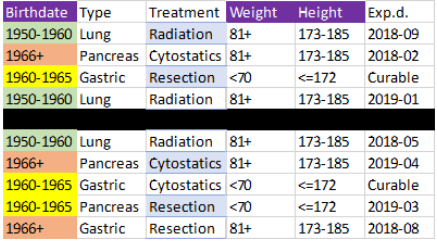
\includegraphics[width=0.6\textwidth]{Assignment0x07/image/anonimyzed_table}
	
	\caption{Anonymized Table}
	\label{img:ano_table}
\end{figure}

\subsection{Explain the homogeneity attack against k-anonymized datasets. Can this be applied to your anonymized dataset? Explain your answer.}

\textbf{Homogeneity Attack}: If all members of a group of k records have the same sensitive data in a column, an attacker can find out that value despite anonymization (it’s always the same, thus predictable). This is hard to avoid completely - our 1950-1960 age group is extremely similar in nearly all respects; thus, an attacker will find out they have lung cancer and are receiving radiation treatment. 
